\documentclass[10pt,twocolumn,letterpaper]{article}

\usepackage{cvpr}
\usepackage{times}
\usepackage{epsfig}
\usepackage{graphicx}
\usepackage{amsmath}
\usepackage{amssymb}
\usepackage{booktabs}
\usepackage{floatrow}

% Include other packages here, before hyperref.

% If you comment hyperref and then uncomment it, you should delete
% egpaper.aux before re-running latex.  (Or just hit 'q' on the first latex
% run, let it finish, and you should be clear).
\usepackage[breaklinks=true,bookmarks=false]{hyperref}

\cvprfinalcopy % *** Uncomment this line for the final submission

\def\cvprPaperID{****} % *** Enter the CVPR Paper ID here
\def\httilde{\mbox{\tt\raisebox{-.5ex}{\symbol{126}}}}

% Pages are numbered in submission mode, and unnumbered in camera-ready
%\ifcvprfinal\pagestyle{empty}\fi
\setcounter{page}{1}
\begin{document}

%%%%%%%%% TITLE

\title{
	Histogram Approach: Deep Learning Texture Analysis \\ 
	\large Methodology}


\author{SSTP Participant\\
Tyler (Taewook) Kim\\
Kent School\\
1 Macedonia Rd., Kent, CT 06757\\
{\tt\small kimt20@kent-school.edu} 
% For a paper whose authors are all at the same institution,
% omit the following lines up until the closing ``}''.
% Additional authors and addresses can be added with ``\and'',
% just like the second author.
% To save space, use either the email address or home page, not both
\and
Grduate Research Assistant\\
Joshua Peeples\\
University of Florida\\
1064 Center Dr, Gainesville, FL 32611\\
{\tt\small jpeeples@ufl.edu}
}

\maketitle
%\thispagestyle{empty}

%%%%%%%%% ABSTRACT
%\begin{abstract}
%   The ABSTRACT is to be in fully-justified italicized text, at the top
%   of the left-hand column, below the author and affiliation
%   information. Use the word ``Abstract'' as the title, in 12-point
%   Times, boldface type, centered relative to the column, initially
%   capitalized. The abstract is to be in 10-point, single-spaced type.
%   Leave two blank lines after the Abstract, then begin the main text.
%   Look at previous CVPR abstracts to get a feel for style and length.
%\end{abstract}

%%%%%%%%% BODY TEXT

%-------------------------------------------------------------------------
\section{Methodology}
%------------------------------------------------------------------------

\subsection{Binning Operation}

Binning operation in standard histogram can be expressed with the following counting fuction:
\begin{equation}
\label{eqn:cf}
y_k = \begin{cases}
1,B_k - w \leq x_k < B_k + w\\
0, otherwise
\end{cases}
\end{equation}

This indicator function returns "1" if the  element falls into a bin and returns "0" else. The condition when an element falls into a bin is defined by $B_k - w \leq x_k < B_k + w$, $B_k$ being the bin center and $w$ being the bin width. However, the standard histogram operation is not differentiable and cannot be used for the backpropagation.\\

Therefore, our approach is to perform a localized binning operation with a sliding window. RBFs will be used instead of standard histogram operation to approximate the count values:


\begin{equation}
\label{eqn:rbf}
y_k =
\cfrac{1}{MN}\sum_{i=1}^{M}\sum_{j=1}^{N}e^{-\cfrac{\left(x_{ij}-\mu_k\right)^2}{\sigma_k^2}}.
\end{equation}


The function above returns the count $y_k$, for kth bin center $\mu_k$ and width $\sigma_k$ from the feature map value $x_{ij}$ .


An example with M$\times$N window in an image is shown in Figure \ref{fig:3_1_1}. Each square represents a pixel with a single intensity value of 1, 2, or 3. Every pixel will contribute to every bin but not equally due to the RBF we are using.

\begin{figure}[H]
	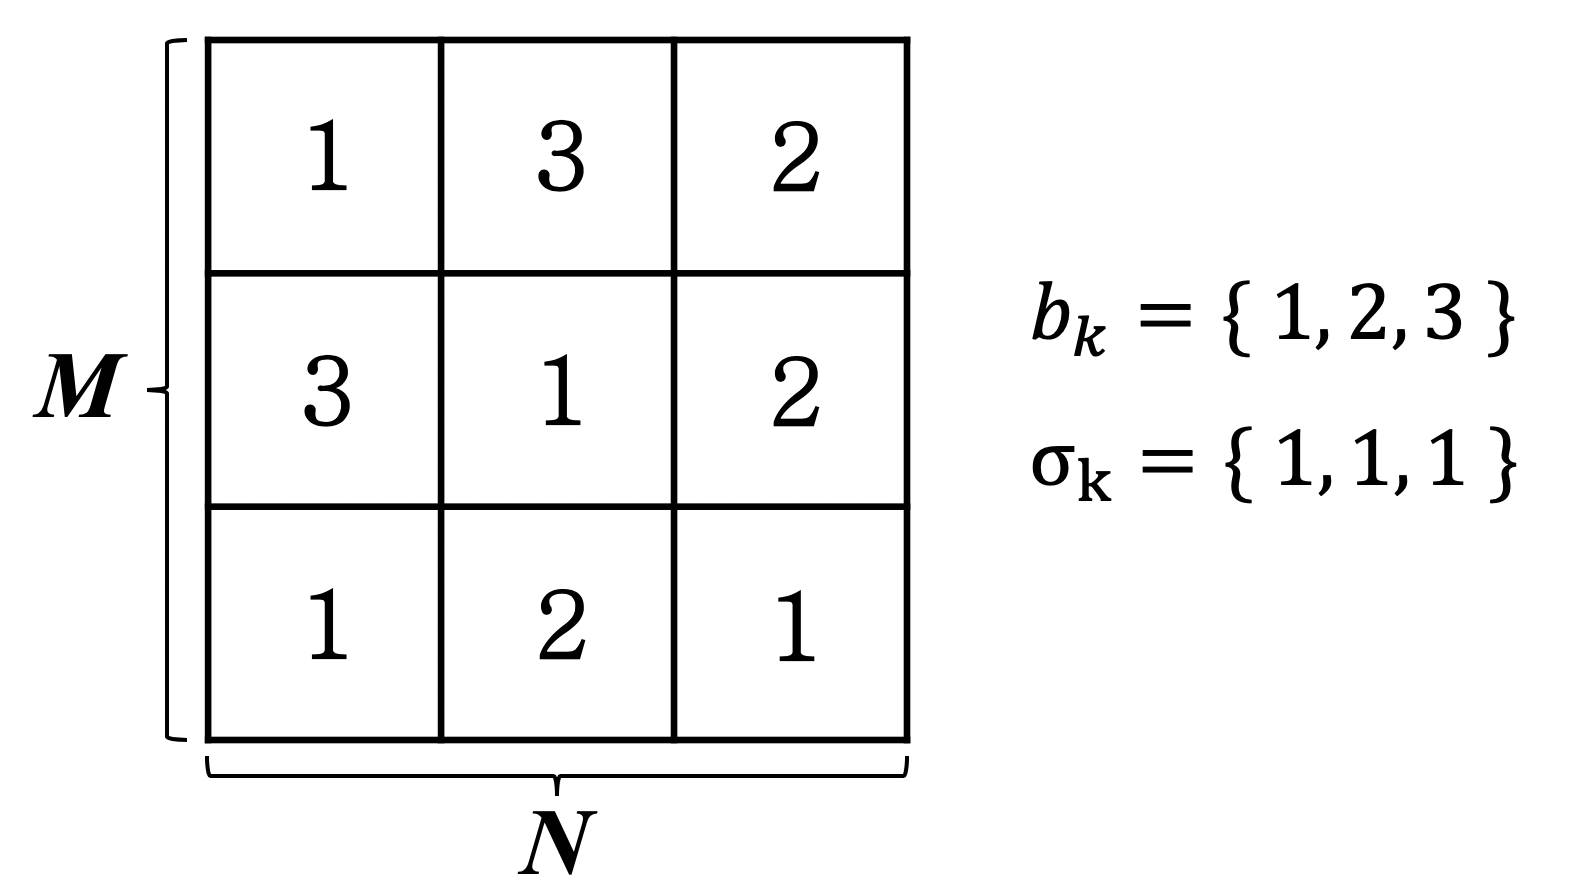
\includegraphics[width=1.0\linewidth]{./Images/3_1_1.png}
	\caption{M$\times$N Window}
	\label{fig:3_1_1}
\end{figure}

\begin{table}[H]
	\begin{tabular}{cccc}
		\hline
		\textbf{} & \textbf{\begin{tabular}[c]{@{}c@{}}$b_0$\\ Value: 1\end{tabular}} & \textbf{\begin{tabular}[c]{@{}c@{}}$b_1$\\ Value: 2\end{tabular}} & \textbf{\begin{tabular}[c]{@{}c@{}}$b_2$\\ Value: 3\end{tabular}} \\ \hline
		Standard & 0.44 & 0.33 & 0.22 \\ \hline
		RBF & 0.57 & 0.42 & 0.35 \\ \hline
	\end{tabular}
	\caption{Normalized Frequency Comparison}
	\label{tab:table1}
\end{table}

Table \ref{tab:table1} compares the resulting count value from the two equations introduced. Each column represents the bins, $b_0$, $b_1$ and $b_2$ each indicating bin center of 1, 2, and 3 respectively. The first row shows the value calculated by \eqref{eqn:cf} with $w = 0$, and the second row is based on \eqref{eqn:rbf}. RBF is used to approximate the counting function because it allows differentiation thereby allowing the model to learn via backpropagation. As shown in Figure \ref{fig:3_1_1}, $\sigma_k$ is set to be 1, which makes the difference between the two values larger. $\sigma_k$ is a crucial factor that determines this difference. As $\sigma_k$ value becomes smaller, the model will only consider the values that are very close to the bin center. If model learns the optimum $\sigma_k$ value, we will be able to account for ambiguity in the data as opposed to crisp histograms. As $\sigma_k$ value becomes larger, every element will fall into the same bin.

\subsection{Experiment Design}

\begin{figure}[H]
	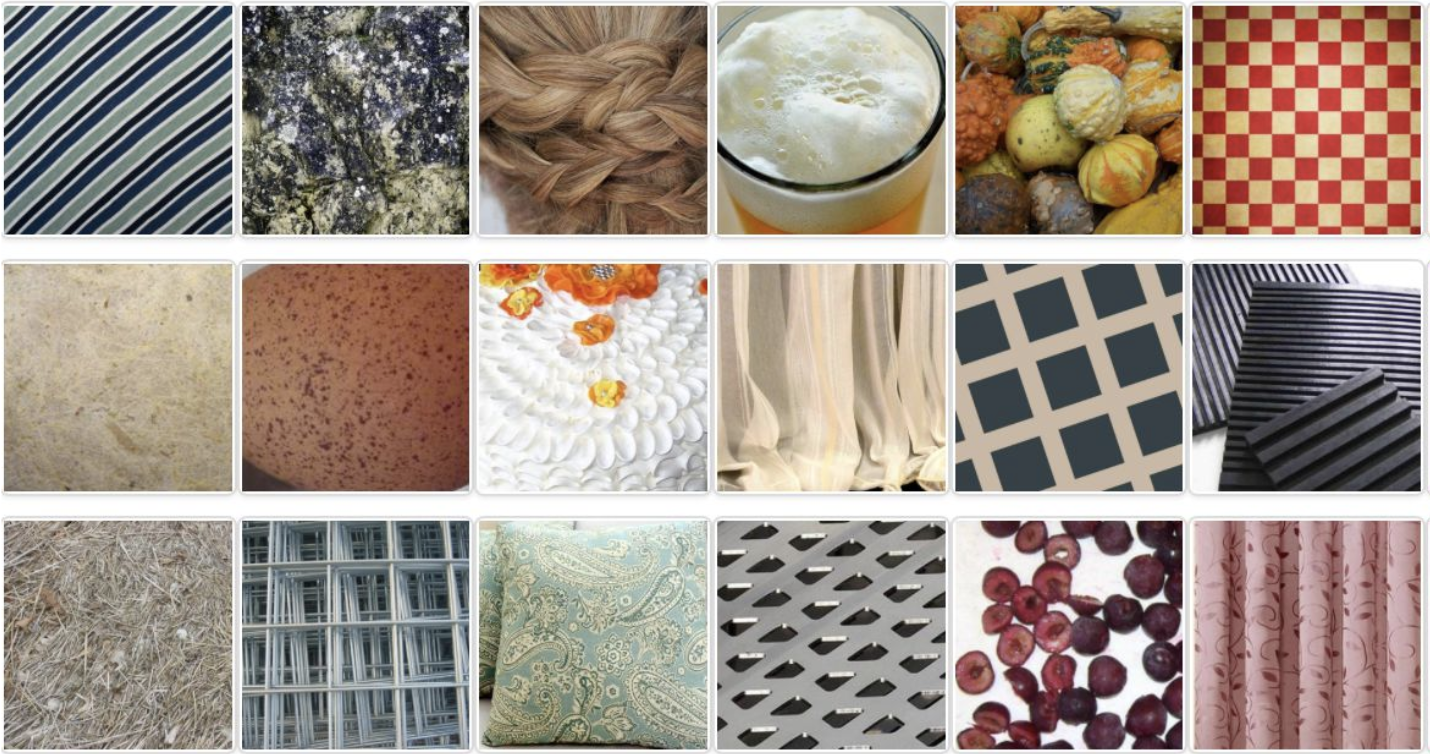
\includegraphics[width=1.0\linewidth]{./Images/3_2_1.png}
	\caption{Example of DTD Images \cite{cimpoi14DTD}}
	\label{fig:3_2_1}
\end{figure}

To evaluate the performance of the proposed model, we used Describable Textures Dataset (DTD), a texture database with 5640 images classified into 47 categories. We will use five different artificial neural networks (ANN) that are comprised of convolutional and histogram layers to classify the images. We will compare the results both quantitatively and qualitatively. In qualitative analysis, we will focus on displaying images that are classified correctly or incorrectly by each network. In quantitative analysis, we record accuracy(class and overall), class precision, class recall, class F1 score, learning curve, and confusion matrices.

\subsection{Training Procedure}
For our training procedure, our data is first scaled to between 0 and 1. Next, we wanted to look at the effects of preprocessing our data through standardization

\begin{equation}
\label{eqn:std}
Z = \dfrac{x - \mu}{\sigma}.
\end{equation}

The equation \ref{eqn:std} represents the standardization operation, where $x$ is the original feature value, $\mu$ is the mean of that feature value, $\sigma$  is its standard deviation, and $Z$ is the resulting standardized data. 
For our dataset, $x$ is the RGB value for each pixel and the corresponding mean ($\mu$) and standard deviation ($\sigma$) for each channel will be used to normalize the data through equation \ref{eqn:std} . Data preprocessing is considered to be one of the most important components of training the model, and we want to compare the results from standardizing the data and relating this to the performance of each network. \\

 
For the training process, we use the same data augmentation and optimization technique for the six different neural networks. Similar to \cite{Xue2018dep}, all the samples were first resized to 256 $\times$ 256 then a crop of random size (0.8 to 1.0) of the original size and a random aspect ratio (3/4 to 4/3) of the original aspect ratio is extracted. This crop is finally resized to 224$\times$224 and horizontal flips ($p=0.5$) were used. The experiment starts with learning rate of 0.01 and batch size of 128. Throughout 100 total epochs, the learning rate decays by factor of 0.9 for every 10 epochs. During the learning rate decay, Adam, an adaptive learning rate optimization algorithm, is used. Adam allows for efficient stochastic optimization that only requires first-order gradients, allowing for little memory requirement\cite{Kingma2014adam}. 


{\small
\bibliographystyle{ieee_fullname}
\bibliography{egbib}
}

\end{document}
